\documentclass[10pt]{article}
\usepackage[utf8]{inputenc}	% Para caracteres en español
\usepackage{amsmath,amsthm,amsfonts,amssymb,amscd}
\usepackage{multirow,booktabs}
\usepackage[table]{xcolor}
\usepackage{fullpage}
\usepackage{lastpage}
\usepackage{enumitem}
\usepackage{fancyhdr}
\usepackage{mathrsfs}
\usepackage{wrapfig}
\usepackage{setspace}
\usepackage{calc}
\usepackage{multicol}
\usepackage{cancel}
\usepackage[retainorgcmds]{IEEEtrantools}
\usepackage[margin=3cm]{geometry}
\usepackage{amsmath}
\newlength{\tabcont}
\setlength{\parindent}{0.0in}
\setlength{\parskip}{0.05in}
\usepackage{empheq}
\usepackage{framed}
\usepackage[most]{tcolorbox}
\usepackage{xcolor}
\usepackage{float}
\usepackage[english]{babel}
\usepackage[utf8]{inputenc}
\usepackage{graphicx}
\usepackage[colorinlistoftodos]{todonotes}
\usepackage[version=4]{mhchem}
\usepackage{physics}
\usepackage{mathtools}
%\DeclarePairedDelimiter\bra{\langle}{\rvert}
%\DeclarePairedDelimiter\ket{\lvert}{\rangle}
%\DeclarePairedDelimiterX\braket[2]{\langle}{\rangle}{#1 \delimsize\vert #2}
%\definecolor{shadecolor}{named}{red!25!green!50!blue!75}
\colorlet{NextBlue}{red!25!green!50!blue!75}
%\colorlet{shadecolor}{orange!15}
\colorlet{shadecolor}{NextBlue!40}
\parindent 0in
\parskip 10pt
\geometry{margin=1in, headsep=0.25in}
\theoremstyle{definition}
\newtheorem{defn}{Definition}
\newtheorem{reg}{Rule}
\newtheorem{exer}{Exercise}
\newtheorem{note}{Note}
\begin{document}
\setcounter{section}{1}
\title{Calculations in perturbation theory}

%==============================================================
\pagestyle{fancy}
\fancyhf{}
\rhead{Physics 180}
\chead{Calculations in perturbation theory}
\lhead{Olyn D. Desabelle}
\rfoot{Page \thepage}
\setlength{\headheight}{12.0pt}

\begin{center}
{\LARGE \bf Calculations in perturbation theory}\\
%{\large Physics 170}\\
%Olyn D. Desabelle
\end{center}

\section*{Spin sums}%----------------------------------------

For a given process, the total amplitude $\mathcal{M}_{fi}$ is the sum of all individual amplitudes (possible Feynman diagrams), but terms aside fromt the matrix element of the lowest-order term are negligible. Including the spin, then the \textbf{spin-averaged matrix element} is given by:

\begin{align}
    \expval{|\mathcal{M}_{fi}|^2} &= \frac{1}{4}\sum_{\text{spins}} |\mathcal{M}|^2\\
    %\expval{|\mathcal{M}_{fi}|^2} 
    &= \frac{1}{4} (|\mathcal{M}_{\text{RR}}|^2 + |\mathcal{M}_{\text{RL}}|^2 + |\mathcal{M}_{\text{LR}}|^2 + |\mathcal{M}_{\text{LL}}|^2)\\
    &= \frac{1}{4} (|\mathcal{M}_{\text{RR}\to\text{RR}}|^2 + |\mathcal{M}_{\text{RR}\to\text{RL}}|^2 + \dots + |\mathcal{M}_{\text{RL}\to\text{RR}}|^2 + \dots)\\
\end{align}

\section*{Helicity amplitudes}%----------------------------------------

We consider an electron-positron annihilation:

\begin{figure}[H]
    \centering
    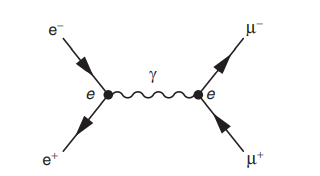
\includegraphics[scale=0.65]{electron positron anal.png}
\end{figure}

For a helicity combination, the matrix element is given by:

\begin{align}
    \mathcal{M} = -\frac{e^2}{s}j_e\cdot j_{\mu}
\end{align}

with the currents given by:

\begin{align*}
    j^0_{\mu} &= \bar{u}_{\uparrow}(p_3)\gamma^0 v_{\downarrow}(p_4)\\
    j^1_{\mu} &= \bar{u}_{\uparrow}(p_3)\gamma^1 v_{\downarrow}(p_4)\\
    j^2_{\mu} &= \bar{u}_{\uparrow}(p_3)\gamma^2 v_{\downarrow}(p_4)\\
    j^3_{\mu} &= \bar{u}_{\uparrow}(p_3)\gamma^3 v_{\downarrow}(p_4)\\
\end{align*}

and each component may be evaluated using: 

\begin{align*}
    \bar{\psi}\gamma^{0}\phi \equiv \psi^{\dagger}\gamma^{0}\gamma^{0}\phi &=
    \psi_1^*\phi_1 + \psi_2^*\phi_2 + \psi_3^*\phi_3 + \psi_4^*\phi_4\\
    \bar{\psi}\gamma^{1}\phi \equiv \psi^{\dagger}\gamma^{0}\gamma^{1}\phi &=
    \psi_1^*\phi_4 + \psi_2^*\phi_3 + \psi_3^*\phi_2 + \psi_4^*\phi_1\\
    \bar{\psi}\gamma^{2}\phi \equiv \psi^{\dagger}\gamma^{0}\gamma^{2}\phi &=
    -i(\psi_1^*\phi_4 - \psi_2^*\phi_3 + \psi_3^*\phi_2 - \psi_4^*\phi_1)\\
    \bar{\psi}\gamma^{3}\phi \equiv \psi^{\dagger}\gamma^{0}\gamma^{3}\phi &=
    \psi_1^*\phi_3 + \psi_2^*\phi_4 + \psi_3^*\phi_1 + \psi_4^*\phi_2\\
\end{align*}



\section*{Trace techniques}

In terms of trace, the sum of matrix element square for all matrices is given by:

\begin{align}
    \sum_{\text{spins}} |\mathcal{M}_{fi}|^2 &= \frac{e^4}{q^4} \mathcal{L}^{\mu\nu}_{(e)}\mathcal{L}^{(\mu)}_{\mu\nu}\\
    &= \frac{e^4}{q^4}\Trace ([\cancel{p}_2-m]\gamma^{\mu}[\cancel{p}_1+m]\gamma^{\nu}) \times \Trace ([\cancel{p}_3+M]\gamma_{\mu}[\cancel{p}_4-M]\gamma_{\nu})
\end{align}

to evaluate the traces, the following theorems are applied:

\begin{figure}[H]
    \centering
    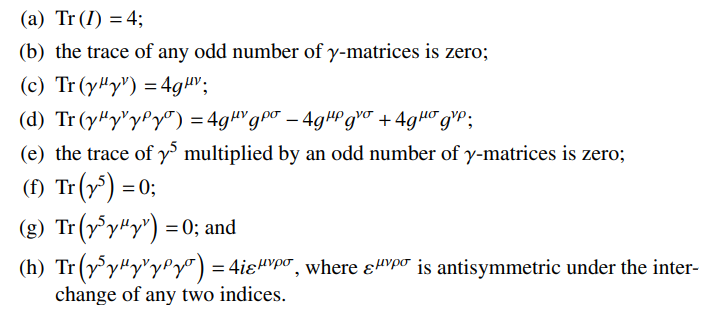
\includegraphics[scale=0.65]{trace.png}
\end{figure}
%----------------------------------------
%----------------------------------------
\end{document}